\section{Realisering og test}
\label{sec:research}

Kretsen i figur \ref{fig:kretsdiagram} ble realisert med komponentene i tabel \ref{tab:comp} vist i figur \ref{fig:realisert}.

\begin{table}[H]
    \centering
    \caption{Komponenter brukt i differensialforsterkeren.}
    \label{tab:comp}
    \begin{tabular}{lll}
    Komponent  & type          & verdi                  \\ \hline
    Q$_1$      & 2N7000        &                        \\
    Q$_2$      & 2N7000        &                        \\
    Q$_3$      & VP2106        &                        \\
    Q$_4$      & VP2106        &                        \\
    Q$_5$      & 2N7000        &                        \\
    Q$_6$      & 2N7000        &                        \\
    R$_{P1}$  &                & \text{20420$\Omega$} \\
    R$_{P2}$  &                & \text{18210$\Omega$}  \\
    R$_{S}$   &                & \text{1k$\Omega$}      \\
    R$_{i1}$  &                & \text{1.2k$\Omega$}    \\
    R$_{i2}$  &                & \text{10.8k$\Omega$}
    \end{tabular}
    \end{table}

\begin{figure}[H]
    \centering
    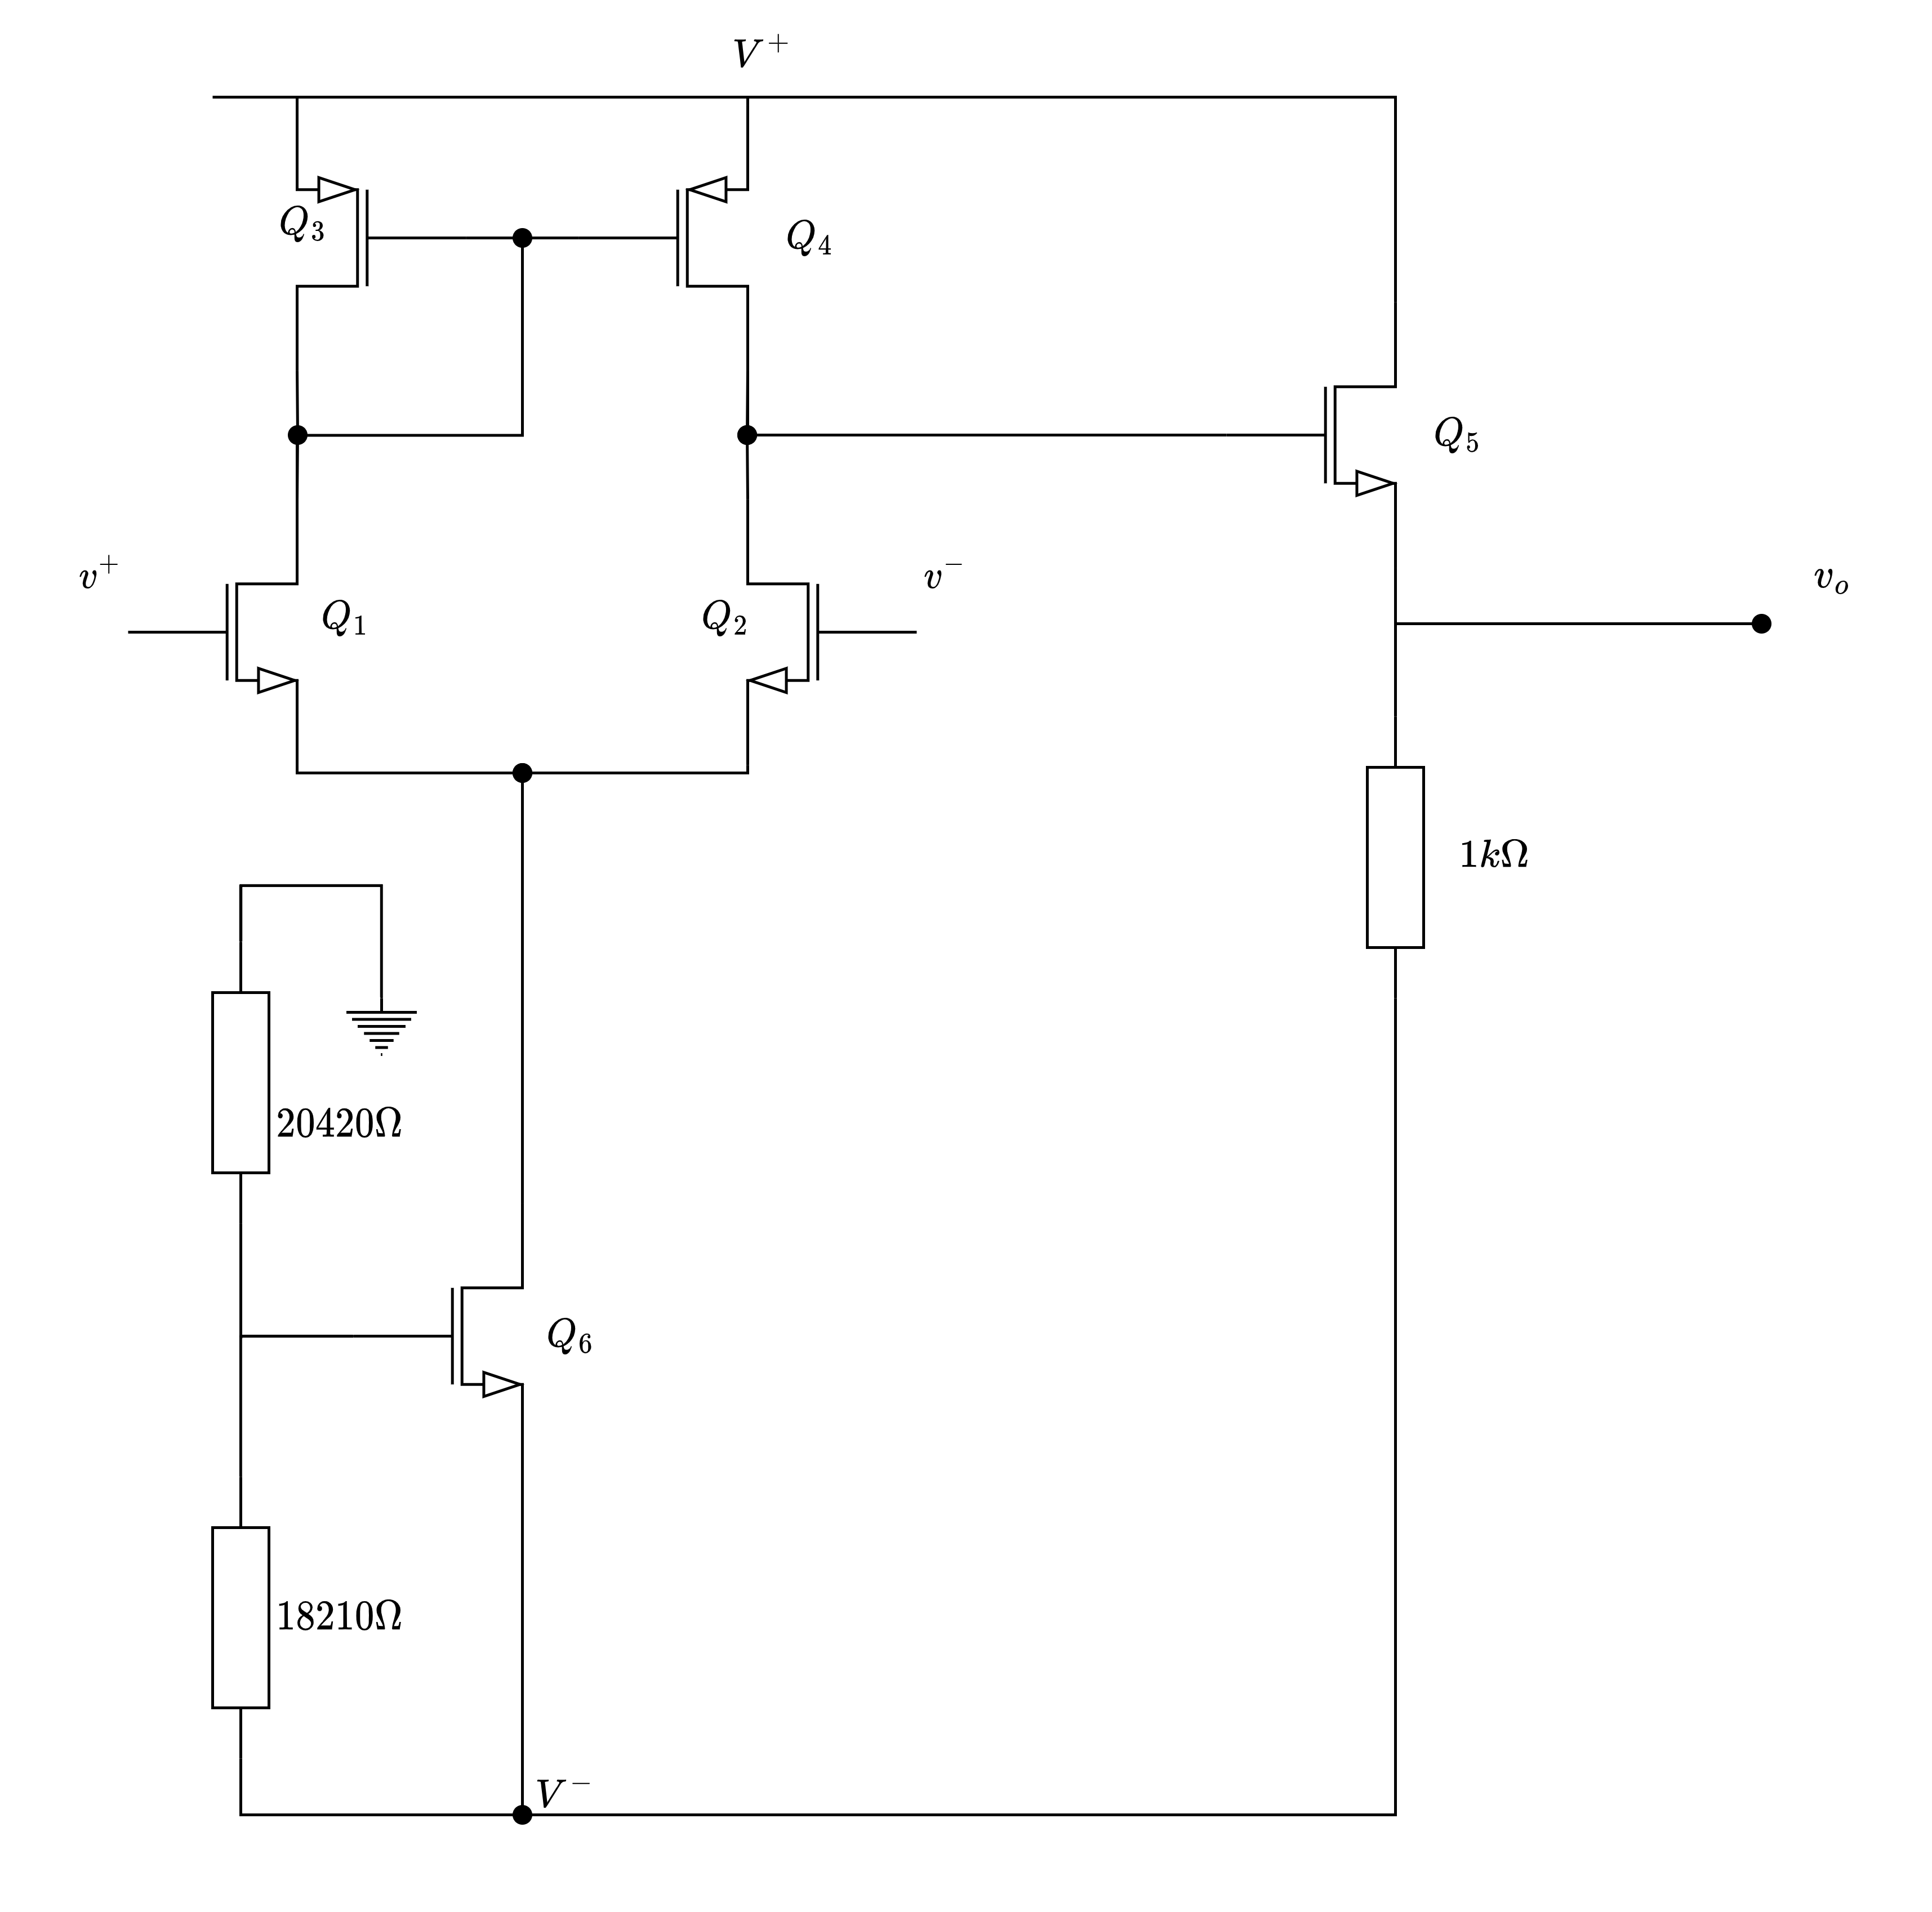
\includegraphics[scale=0.1]{./Images/03Research/full kretes.drawio.png}
    \caption{Realisert krets.\cite{pham_2022_selvlaget}|}
    \label{fig:realisert}
\end{figure}

\begin{figure}[H]
    \centering
    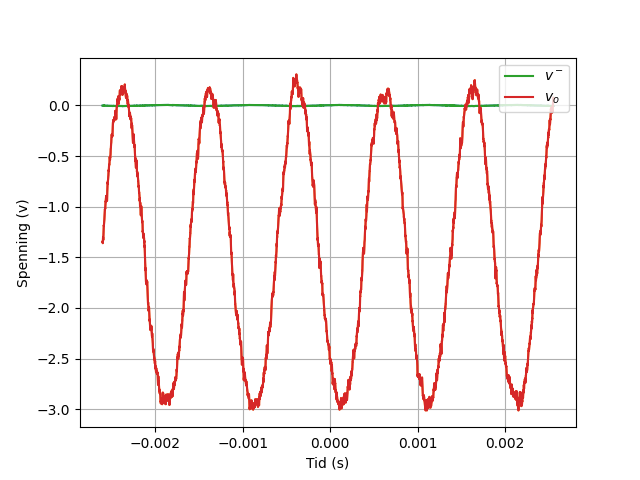
\includegraphics[scale=0.5]{./Images/03Research/åpenløkkeplain.png}
    \caption{Åpen-løkkeforsterkning med en inngangssignal på 5mV.}
    \label{fig:åpenløkke}
\end{figure}

    Ved å sende in et sinussignal med en frekvens på 1kHz med 5mV i amplitude på $v^-$, så ble det målt en forsterkning på $A \approx 350$ og en THD på $-27.6dB$ signalet er vist i figur \ref{fig:åpenløkke}. Det ble også observert lavere forsterkning og høyere THD dersom amplituden på inngangssignalet ble økt fram til 10mV da det ble observert klipping i utgangssgnalet som vist i figur \ref{fig:åpenløkke15mv}. Dermed så blir sinussignalet med 5mV i amplitude brukt videre i prosjektet. 

    \begin{figure}[H]
        \centering
        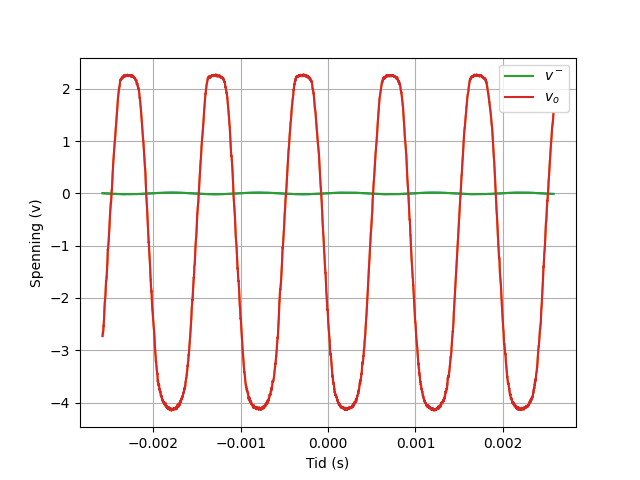
\includegraphics[width=.6\linewidth]{./Images/03Research/åpenløkkeplain15mv.png}
        \caption{Åpen-løkkeforsterkning med en inngangssignal på 15mV.}
        \label{fig:åpenløkke15mv}
    \end{figure}

Dette kan skyldes at det ikke er tilstrekkelig med spenningsforsyning $V^+$ og $V^-$ da tilsvarende klipping også forekom ved en inngangssignal på 5mV når spenningsforsyningen ble redussert.

Måling av THD og forsterkning $A$ ved sinuspåtrykk med frekvens f = 1 kHz med både 100 \text{$\Omega$} og 100 k\text{$\Omega$} er plottet inn i tabell \ref{tab:lastmotstand} der utgangssignalene er vist i figur \ref{fig:åpenløkker} og oppsettet vist i figur \ref{fig:testeer}

\begin{table}[H]
    \centering
    \caption{Forsterkning og THD ved ulik last motstand og type måling.}
    \label{tab:lastmotstand}
    \begin{tabular}{llll}
    Type                & $R_L$                & A      & THD[dBc]     \\ \hline
    Åpen-løkke          & 0                    & 348    & -36.7        \\
    Åpen-løkke          & 100 \text{$\Omega$}  & 91     & -7.7         \\
    Åpen-løkke          & 100 \text{$K\Omega$} & 346    & -37.0        \\
    Ikke-inverterende   & 100 \text{$\Omega$}  & 9.74   & -48.01       \\
    Ikke-inverterende   & 100 \text{$K\Omega$} & 9.83   & -59.85      
    \end{tabular}
    \end{table}

    \begin{figure}[H]
        \centering
        \begin{subfigure}{.5\textwidth}
            \centering
            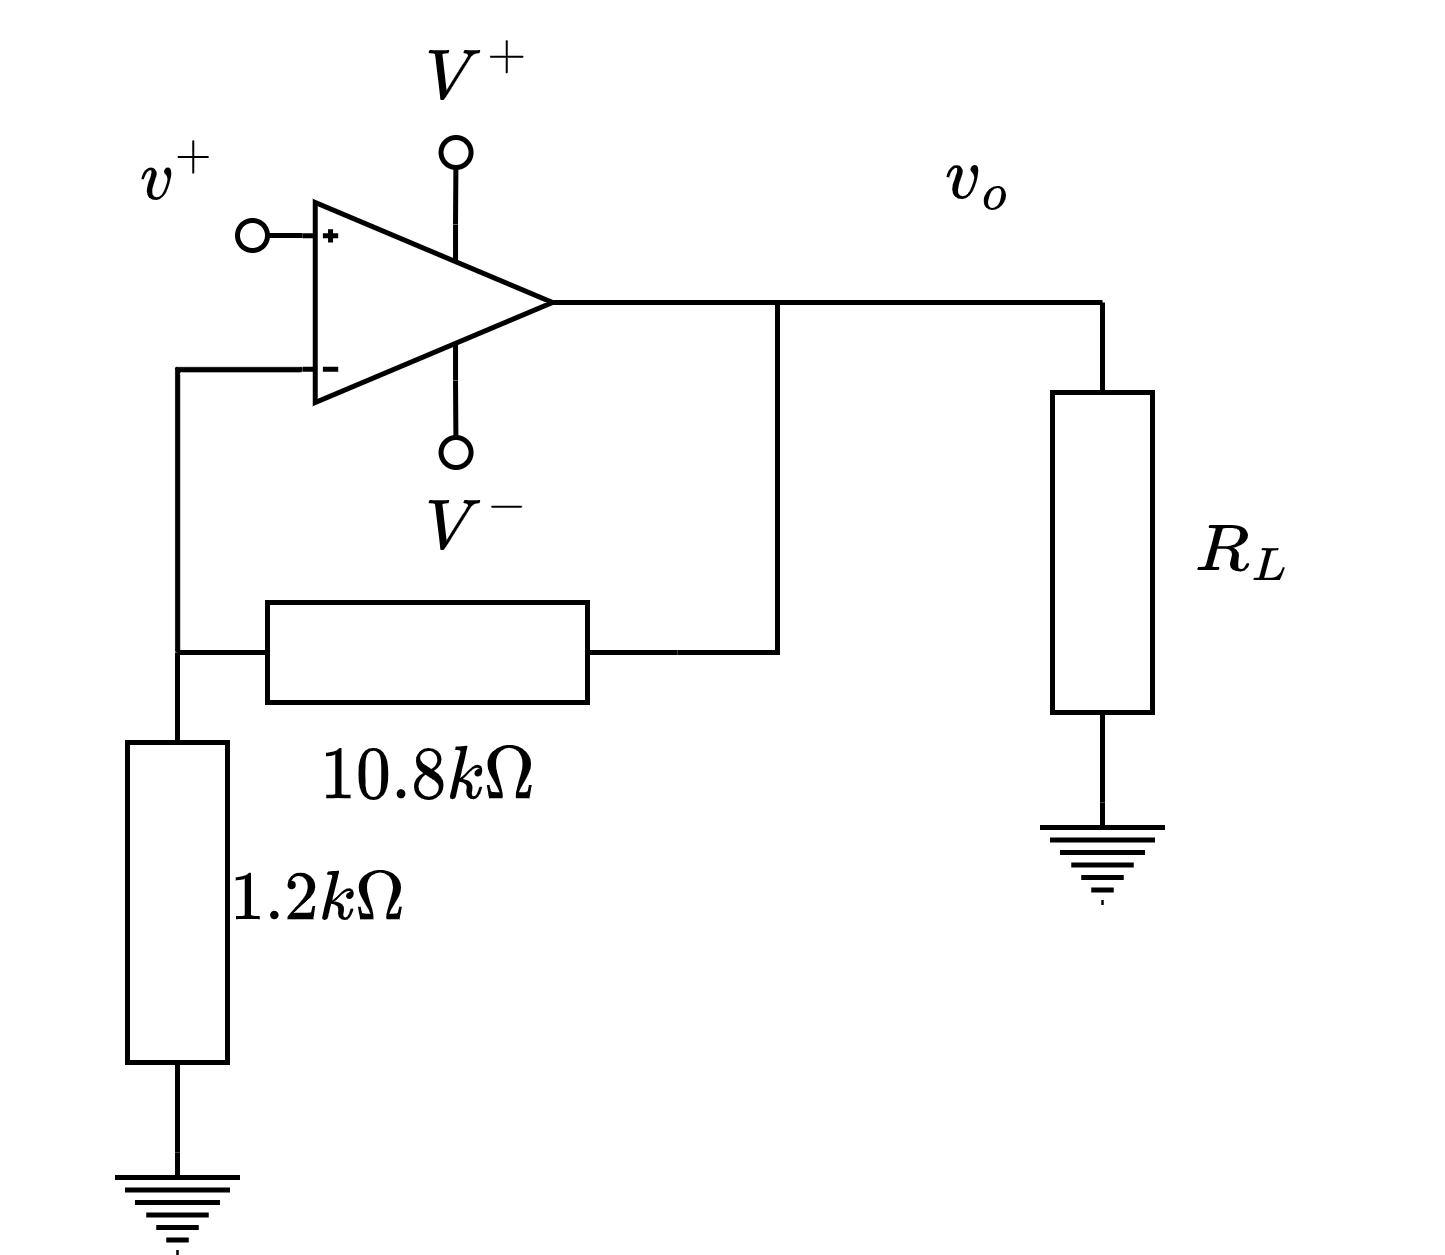
\includegraphics[width=1\linewidth]{./Images/03Research/opamp.drawio.png}
            \caption{Ikke-inverterende forsterker med forskjellig $R_L$}
            \label{fig:ikkeinver}
        \end{subfigure}%
        \begin{subfigure}{.5\textwidth}
            \centering
            \includegraphics[width=1\linewidth]{./Images/03Research/åpenklr.png}
            \caption{Åpen-løkke med lastmotsand $R_L$}
            \label{fig:åpenmløkke}
        \end{subfigure}
        \caption{\cite{pham_2022_selvlaget}}
        \label{fig:testeer}
    \end{figure}

    \begin{figure}[H]
        \centering
        \begin{subfigure}{.5\textwidth}
            \centering
            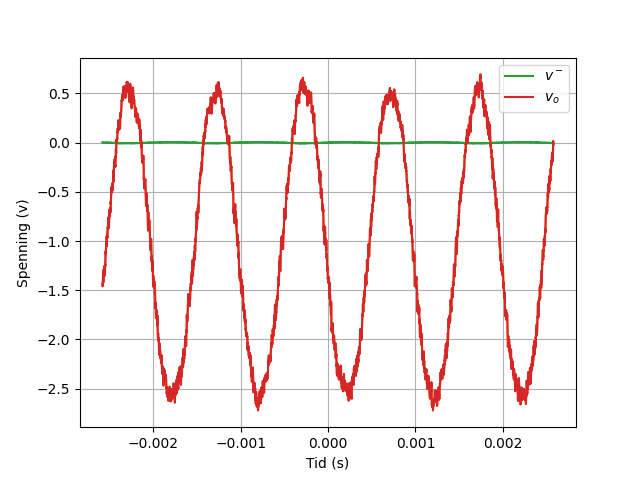
\includegraphics[width=1\linewidth]{./Images/03Research/åpenløkkeplain100kohm.png}
            \caption{Åpen-løkkeforsterkning med lastmotsand på 100k{$\Omega$}}
            \label{fig:100k}
        \end{subfigure}%
        \begin{subfigure}{.5\textwidth}
            \centering
            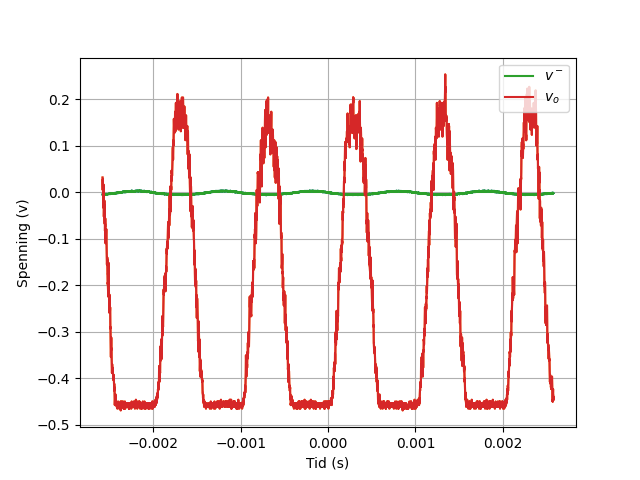
\includegraphics[width=1\linewidth]{./Images/03Research/åpenløkkeplain100ohm.png}
            \caption{Åpen-løkkeforsterkning med lastmotstand på 100{$\Omega$}}
            \label{fig:100}
        \end{subfigure}
        \caption{}
        \label{fig:åpenløkker}
    \end{figure}

    Siden spenningen blir lavere over lastmotstanden \text{$R_L$} ved lav motstand kan det tenkes at utgangsmotstanden  til systemet har noe å si da det skjer et spenningsfall før lastmotstanden i motsetning til en høy lastmotsand da tilnermet alt spenningsfallet skjer over denne.

    \begin{figure}[H]
        \centering
        \begin{subfigure}{.5\textwidth}
            \centering
            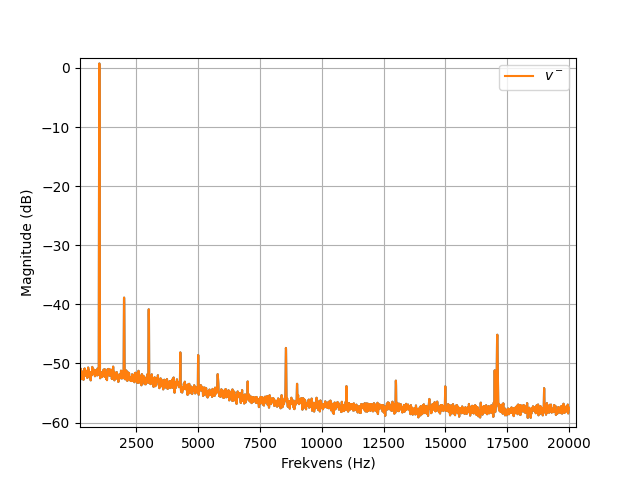
\includegraphics[width=1\linewidth]{./Images/03Research/spektrum100k.png}
            \caption{Åpen-løkkeforsterkning med lastmotsand på 100 k$\Omega$}
            \label{fig:100kspek}
        \end{subfigure}%
        \begin{subfigure}{.5\textwidth}
            \centering
            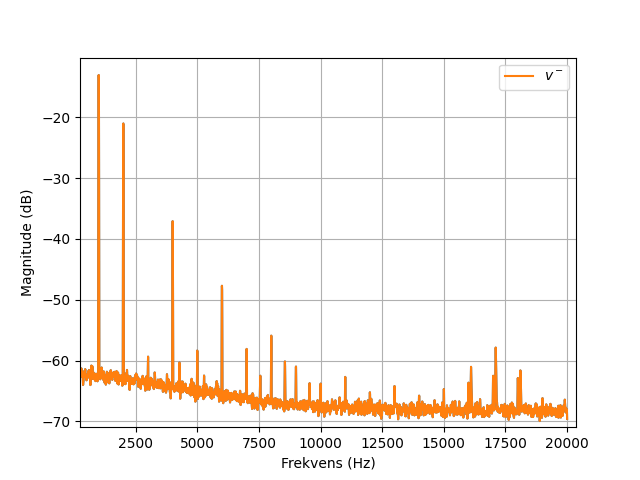
\includegraphics[width=1\linewidth]{./Images/03Research/spektrum100.png}
            \caption{Åpen-løkkeforsterkning med lastmotsand på 100$\Omega$}
            \label{fig:100spekk}
        \end{subfigure}
        \caption{Frkvensspekter for lastmotsand på 100 k\text{$\Omega$} og 100 \text{$\Omega$}}
        \label{fig:Frkvensspekter}
    \end{figure}

Det er observert at lav lastmotstand også gir mer overharmonisk støy i figur \ref{fig:100spekk}.

Ved ikke-inverterende forsterkerkobling som vist i figur \ref{fig:ikkeinver} med en forsterkning $A \approx 10$ ble utgangssignalene seende som vist i figur \ref{fig:ikkeinv}, mens frekvensspekteret er plottet i figur \ref{fig:ikkeinvspek}. Da det er lavere forsterkning her så blir det brukt en høyere amplitude på inngangssignalet. Det er lite forskjell på forsterkning mellom høy og lav lastmotstand, men det forekommer mer støy på den ikke-inverterende forsterkerkoblingen med lav lastmotstand. Til tross for dette så er det generelt lavere støy og forsterkningene på 9.74 og 9.83 ganske så nerme 10, da forholdet mellom ${R_{I2}}$ og ${R_{I1}}$ ifølge formelen \ref{eq:ikkeinv} skal føre til en forsterkning A=10.


\begin{figure}[H]
    \centering
    \begin{subfigure}{.5\textwidth}
        \centering
        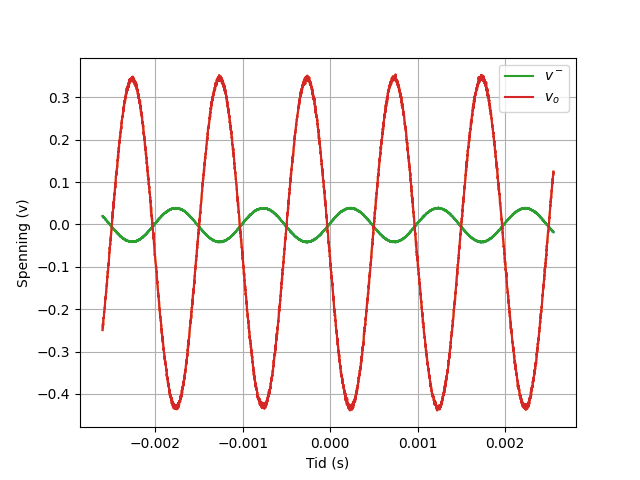
\includegraphics[width=1\linewidth]{./Images/03Research/noninverting100k.png}
        \caption{Ikke-inverterendeforsterkning med lastmotsand på 100 k\text{$\Omega$}}
        \label{fig:ikkeinv100k}
    \end{subfigure}%
    \begin{subfigure}{.5\textwidth}
        \centering
        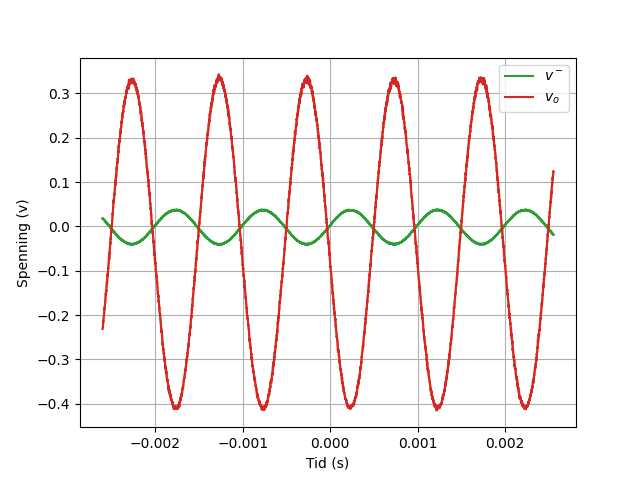
\includegraphics[width=1\linewidth]{./Images/03Research/noninverting100.png}
        \caption{Ikke-inverterendeforsterkning med lastmotsand på 100 \text{$\Omega$}}
        \label{fig:ikkeinv100}
    \end{subfigure}
    \caption{Ikke-inverterendeforsterkning med inngangssignal på 40mV.}
    \label{fig:ikkeinv}
\end{figure}

\begin{figure}[H]
    \centering
    \begin{subfigure}{.5\textwidth}
        \centering
        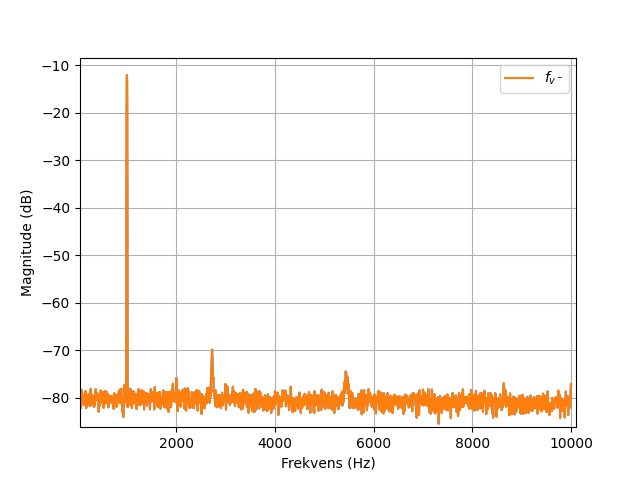
\includegraphics[width=1\linewidth]{./Images/03Research/noninvertingspektrum100k.png}
        \caption{Frekvensspekter med lastmotsand på 100 k\text{$\Omega$}}
        \label{fig:ikkeinvspek100k}
    \end{subfigure}%
    \begin{subfigure}{.5\textwidth}
        \centering
        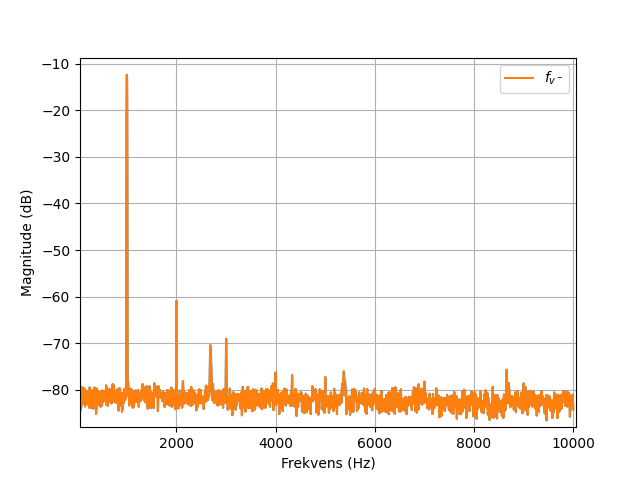
\includegraphics[width=1\linewidth]{./Images/03Research/noninvertingspektrum100.png}
        \caption{Frekvensspekter med lastmotsand på 100 \text{$\Omega$}}
        \label{fig:ikkeinvspek100}
    \end{subfigure}
    \caption{Frekvensspekter til ikke-inverterendeforsterkning med inngangssignal på 40mV.}
    \label{fig:ikkeinvspek}
\end{figure}

For å finne uv av inngangs- og utgangshastigheten blir metoden i dokumentet \cite{ntnu_2022_ttt4265} brukt, der ved måling av inngangsmotstanden R$_i$ blir gjort ved å legge til en kjent motstand R' = 1M$\Omega$ som vist i figur \ref{fig:lastmot}

\begin{figure}[H]
    \centering
    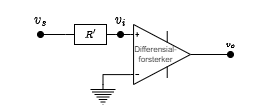
\includegraphics[scale=0.1]{./Images/03Research/lastmot.png}
    \caption{måling av inngangsmotstand.\cite{pham_2022_selvlaget}}
    \label{fig:lastmot}
\end{figure}

der formelen for inngangsmotstanden er gitt ved

\begin{equation}
    R_i=R'\frac{v_i}{v_s}
\end{equation}

Her er For å måle inngangsmotstanden ble det brukt en lastmotstandmotstand på 1M$\Omega$ i figur \ref{fig:lastmot}, $v_i$ ble målt til 69mV, og $v_s$ ble målt til 42mV. Dette gir en inngangsmotstand på $R_i\approx$1.55M$\Omega$.

\begin{figure}[H]
    \centering
    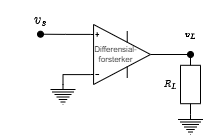
\includegraphics[scale=0.1]{./Images/03Research/outmot.png}
    \caption{måling av utgangsmotstand.\cite{pham_2022_selvlaget}}
    \label{fig:outmot}
\end{figure}

Ved måling av utgangsmotstanden ble en motstand $R_{LO}$ brukt som vist i figur \ref{fig:outmot} der spenningen $v_o$ målt før motstanden ble satt på ble målt til 3.276V, mens $v_L$ ble målt til 1.37V. Motstanden som ble brukt var på 100$\Omega$ dermed ved bruk av formelen i dokumentet \cite{ntnu_2022_ttt4265} så gir det en utgangsmotstand på $R_o\approx$129$\Omega$.

\begin{equation}
    R_o=R_{LO}\frac{v_o-v_L}{v_L}
\end{equation}

Den fysisk oppkoblet kretsen er vist i figur \ref{fig:fysisk}
\begin{figure}[H]
	\centering
	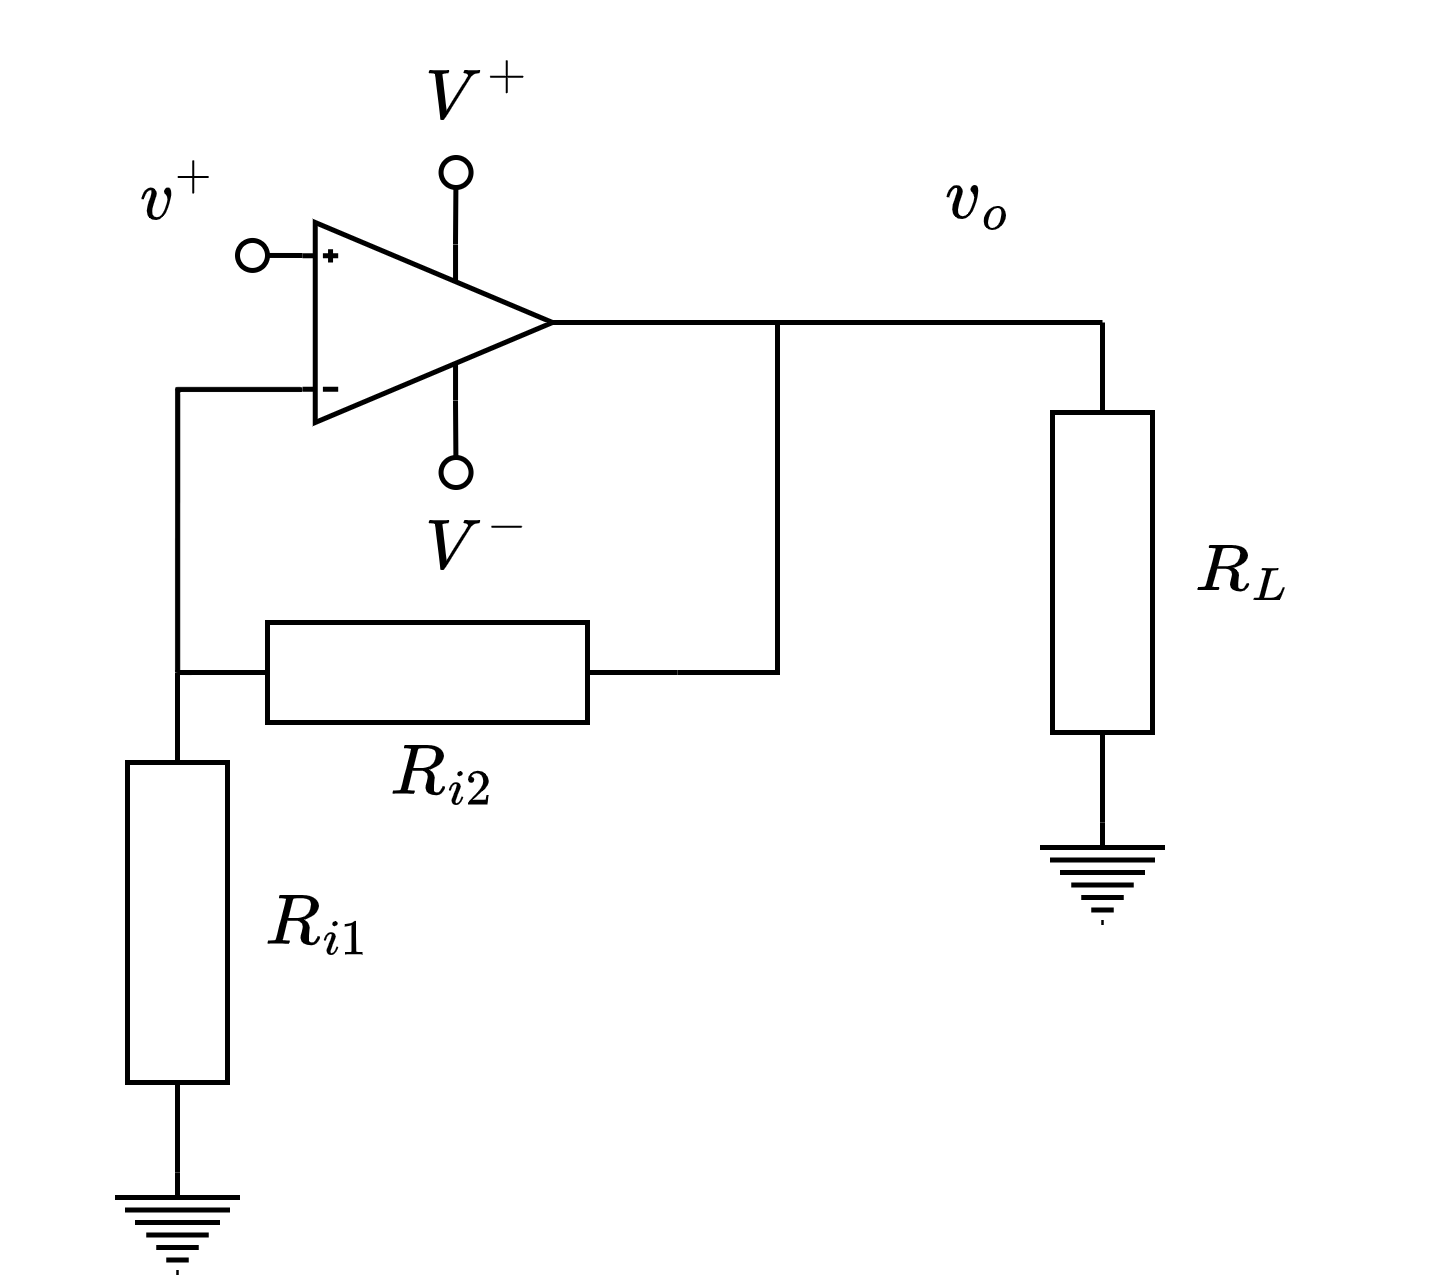
\includegraphics[scale=0.2]{./Images/03Research/ikkeinverterende.png}
	\caption{Fysisk oppkoblet krets.}
	\label{fig:fysisk}
\end{figure}



